\documentclass[12pt]{article}
\bibliographystyle{plain}
\usepackage{graphicx}
\usepackage{lipsum}
\usepackage[margin=1in]{geometry} % sets margin size
\usepackage[section]{placeins} % prevents figures from separating from their sections
\usepackage{hyperref}
\title{System Communication: Real-Time Data Transport Prototype}
\author{L. Callahan, N. DePergola, A. Kaufmann,\\D. Lalli, T. Matson, T. Nguyen}
\date{October 2026}
% Defining the document setup and imports above
% Use the percent sign to make comments in LaTeX

\begin{document}
\maketitle % importing the title we defined above.

% Adding this line break === between sections for clarity
%=====================================================================================

\section*{Abstract}

\*Interferometers used in Radio Astronomy require real time communication between antenna sites and new instruments, such as the ngVLA, and ngRadar would strongly benefit from system communication between observation planning, telescope control, and data transport software. Currently, there is no direct connection between these software components and NRAO personel must communicate directly to plan observations across sites.
This software documents a real-time data transport architecture developed by the NRAO, and demonstrates a possible use in the future ngRadar system, but could be implemented into any radio astronomy observatory. The software architecture is entirely event-driven while each event is also saved in a central database, with every event visible to users on a public website. The prototype has been tested with simulated observation data, and has demonstrated the ability to work remotely across geographically located sites. 

%=====================================================================================

\section{Introduction}
The ngRadar system will utilize the Green Bank Telescope as a high powered transmitter, capable of transmitting a 13.7 GHz frequency at 500kW, and be able to image objects 10 times farther than the lunar distance. The Very Long Baseline Array (VLBA) will be used to receive those signals, before being sent to the Domenici Science Operations Center (DSOC) for data processing. During test observations with the low powered transmitter, scientific staff had to communicate over the phone with telescope operators across the GBT and VLBA sites to coordinate planned observations, including observation targets and times.

The Real-Time System Communication Prototype was developed to demonstrate system communications between remote NRAO locations. This paper documents an event-driven, web-based application for remote viewing of an active observation across geographically dispersed sites. Although this software could be implemented on many NRAO observatories, the ngRadar system was chosen for our team to demonstrate the prototype's proof of concept.

This memo details the design decisions (Section V), system architecture decisions (Section II), software components and technologies chosen (Section III), and other dependencies required by the System Communication Prototype (Section IV).

%=====================================================================================

\section{System Architecture}

\hspace{0.5cm} To enable system communication across different NRAO sites, the software would need to be compatible with various types of computers and operating systems used by NRAO personel - Windows, Linux, and MacOS. For use in ngRadar, the software would need to communicate across the continental United States, Hawaii, and the Caribbean. 
    
  The team initially investigated developing software which would be installed locally on the computers of NRAO employees, and transmit data over the internet to the software at other locations. However, this would have required compiling and building an application for all three major operating systems. Therefore, it was decided that the software would not be locally hosted, and instead function as a web application. This website would be primarily hosted on servers at DSOC, with other software components hosted at the Green Bank Observatory and on all 10 of the VLBA sites. For end-to-end communication online, Apache Kafka was chosen as the message broker because of its reliability, scalability, and use across a wide range of industries. Both locally hosted and web hosted versions of Kafka have been tested in this software prototype, but a locally hosted Kafka message broker was chosen as the more viable option; this option provides a lower cost, increased flexibility, and direct control of data transmitted over the website. To manage server and back-end logic, the Django web framework was chosen due to the large number of compatible software libraries, built in security and adminstrative features, and its ability to scale as website traffic grows.

  While Apache Kafka is responsible for sending and receiving event notifiers on the website, another software tool must be used to send the actual observation data from the receiving antennas to DSOC. The team investigated two different tools for the movement of observation data. The first tool demonstrated with this software is E-transfer, an open source client/daemon used for high speed data transfers and developed by the Joint Institute for Very Long Baseline Interferometry European Research Infrastructure Consortium (JIVE). Additionally, the team demonstrated ExpeDat, a data transfer tool which utilizes a proprietary file transport protocol based on UDP. ExpeDat was developed by Data Expedition inc, and the software is available as a free trial or for purchase with a one time fee. Due to project time contraints, the team spent 8 weeks using E-transfer for transmitting observation data, but only 2 weeks using ExpeDat. However, data collected on the performance of these tools showed \textbf{[fill in later]} consistently worked faster.
  
  This web application did not make use of a dedicated front-end framework, and instead used HTML pages supported by Javascript, CSS, and bootstrap code. To store and display information generated by the simulated observation events, an SQL database was used. PostgreSQL was chosen because it is open source, free, and widely used across tech companies. The database is hosted at the simulated DSOC location within our software prototype. It should be noted that while the database is responsible for storing the history of observed events, the database is not required for the website to function, as it is entirely driven by Kafka message events.

  Security was an important consideration during the development process - if a web application with similar design architecture is implemented for actual use in ngRadar, it will run directly on NRAO computers across numerous observatory locations, and potentially interface with telescope hardware. Docker Containers play a role in keeping local computers safe, since applications within them are isolated from the rest of the computer. Django also has several built in security features, including user authentication, cross site scripting, and forgery attack protection.

  During the development process, the team needed a way to ensure that this website could be run across multiple machines for local development and debugging, but also perform reliably when run on a cloud-based or locally hosted server. To accomplish this, we used Docker Containers to isolate software components and their dependencies used on our website. This would ensure that any computer which has the Docker Engine - a server responsible for managing the containers - can run this web application and it will perform consistently.
  
\vspace{5mm} Fig. \ref{fig:step1} shows the first step of the system sequencing. The user submitting a new waveform indicates the beginning of the process, which triggers the initial Kafka message. An arrow from A to B represents a Kafka message produced by A and consumed by B. 

\begin{figure}[h!] 
\centering 
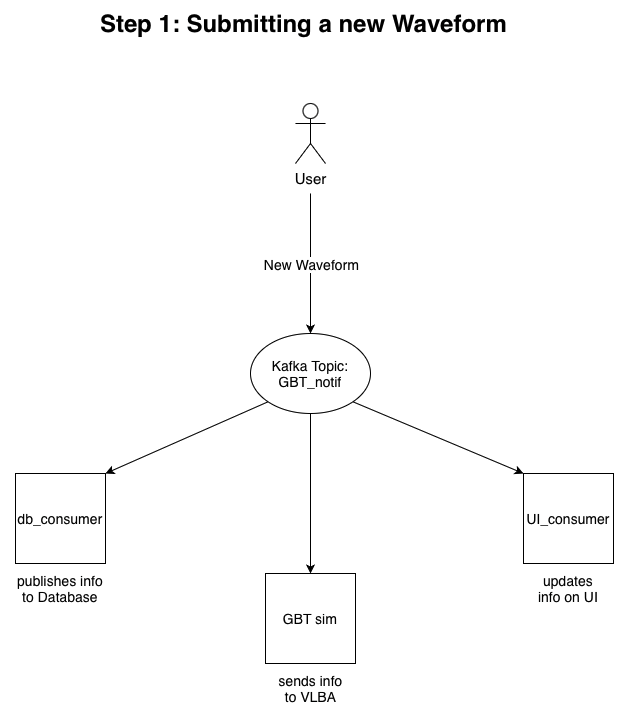
\includegraphics[width=0.65\columnwidth]{Step1_sequence.png} 
    \caption{*\textbf{Note for team}: the quality of this image is bad. We can replace it once we agree if we want to use it!} 
    \label{fig:step1}
\end{figure}

\begin{figure}[h!] 
\centering 
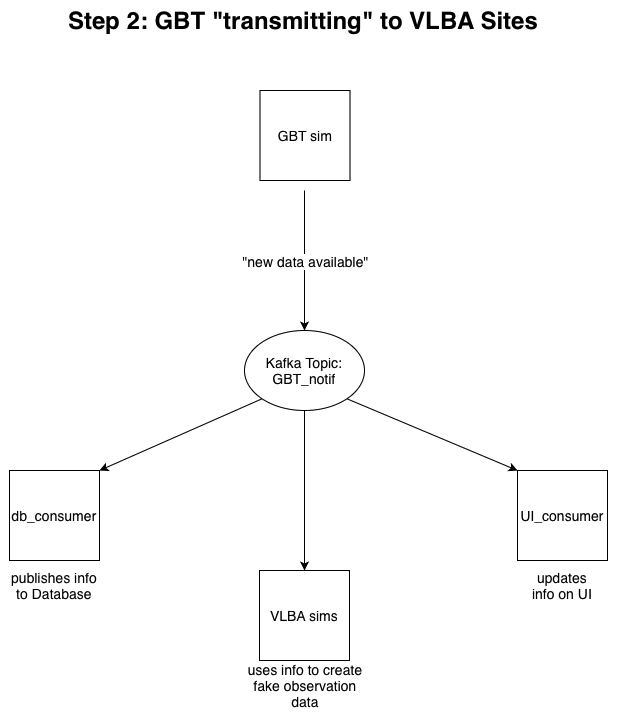
\includegraphics[width=0.65\columnwidth]{Step2_sequence.png} 
    \caption{*\textbf{Note for team}: the quality of this image is bad. We can replace it once we agree if we want to use it!} 
    \label{fig:step2}
\end{figure}

\begin{figure}[h!] 
\centering 
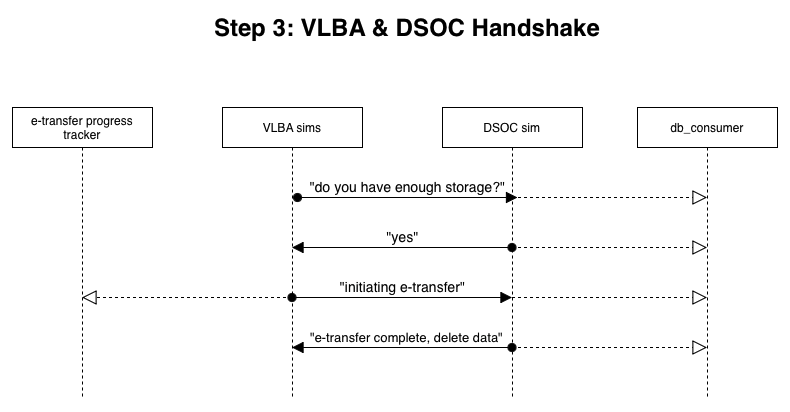
\includegraphics[width=0.65\columnwidth]{Step3_sequence.png} 
    \caption{*\textbf{Note for team}: the quality of this image is bad. We can replace it once we agree if we want to use it!} 
    \label{fig:step3}
\end{figure}

%=====================================================================================

\section{Software Stack}

\subsection*{Django}

Python is widely used across astronomy, all team members had prior experience coding in it, and our website did not require the extra computing speed offered by compiled languages such as C++, so the team chose to use a python framework. There were three frameworks our team investigated - Flask, FastAPI, and Django. 
  Flask is well-known for its simplicity and low usage of computing resources. It is also flexible and modular, allowing developers to modify the framework and integrate additional software components for added functionality. However, Flask only supports using synchronous communication between the server and framework, meaning processes can only run one-at-a-time. Flask does not have built in authentication or adminstrative features, and this prototype website would benefit from non-blocking communication.
  FastAPI provides high-speed, and asynchronous, non-blocking communication in a relatively lightweight framework. It is the newest framework we investigated and includes features such as built in authentication, python code completion to speed up development, and automatic documentation for program APIs. It includes a modest number of built in functionality, and developers can add libraries with additional features they need.
  Django is a framework with a large amount of built in functionality including an adminstrative dashboard, user authentication, HTML form processing, and an object-relational mapper for database interaction [Revisit and add any additional built-in features we used]. It is capable of running large web applications with many users. By default, Django runs with synchronous communication, but libraries that add asynchronous communication are avaliable.


\url{https://nrao.atlassian.net/wiki/spaces/DOB/pages/1112277010/Back-End+Frameworks?atlOrigin=eyJpIjoiYTk2NmMwOTI0MjYyNGEzNDliZTYzODVmYTc0MmJiMTMiLCJwIjoiYyJ9}

\url{https://nrao.atlassian.net/wiki/spaces/DOB/pages/1114275857/Web+Applications+for+Beginners?atlOrigin=eyJpIjoiZjBlZGU5NWFkNzRjNDFjMThkNWVlMTVjOGZkZjU0NTkiLCJwIjoiYyJ9}

\url{https://nrao.atlassian.net/wiki/x/C4DlUQ}

\url{https://nrao.atlassian.net/wiki/spaces/DOB/embed/1146814469}
\url{https://nrao.atlassian.net/wiki/x/C4DlUQ}
\subsection*{Docker}
In this software prototype, the team 

\url{https://nrao.atlassian.net/wiki/x/AYCtPw}
\url{https://nrao.atlassian.net/wiki/x/AQDFSg}

\subsection*{Apache Kafka}

\url{https://nrao.atlassian.net/wiki/x/HYA-Pg}

\url{https://nrao.atlassian.net/wiki/x/AYBTUg}

\subsection*{PostgreSQL}


\subsection*{E-Transfer}

\url{https://nrao.atlassian.net/wiki/x/GQBoRw}

\url{https://nrao.atlassian.net/wiki/x/AQDRS}

\url{https://nrao.atlassian.net/wiki/x/AQAZSg}

\url{https://nrao.atlassian.net/wiki/x/HABRV}

\subsection*{ExpeDat}

\subsection*{SeaweedFS}

\url{https://nrao.atlassian.net/wiki/x/GgAMRQ}

\url{https://nrao.atlassian.net/wiki/x/CYBfRw}

\subsection*{DigitalOcean}

\url{https://nrao.atlassian.net/wiki/x/BoDsT}

\url{https://nrao.atlassian.net/wiki/x/BACsTg}

\url{https://nrao.atlassian.net/wiki/x/AYAqUg}


\subsection*{Monitoring Tools}

\subsubsection*{Traefik}

\subsubsection*{Grafana}

\subsubsection*{Prometheus}

\subsubsection*{k6}

\subsubsection*{OpenTelemetry}

%=====================================================================================

\section{Dependencies}


%=====================================================================================
\section{Design Decisions}


%=====================================================================================
\section{Ideas for Future Improvements}
\begin{itemize}
  \item Features
  \begin{itemize}
    \item Originally, DSOC checks its storage and responds to a single VLBA station if it can accept the incoming e-transfer/expedat raw data transfer/stream. Currently, we have this check occurring simultaneously for all 10 VLBA stations. But we noticed that with 10 consecutive storage check requests, DSOC responds yes without taking into account the requests it’s already approved. With the simultaneous transfers/streams, DSOC storage could potentially go over its storage limit for incoming raw data. It would be beneficial to have some logic built in place for DSOC to keep track of its storage before and after each approval of a requested VLBA site's incoming transfer/stream.
    \item Currently, on our history events page, you can see that in our sequencing of events, DSOC sends a 'Completed' kafka message 10 times per 10 VLBA sims. It might make more sense to have DSOC wait until it has finished processing all 10 VLBAs raw data, generates its 10 DDM images and stores them to seaweedfs, and then send only one 'Completed' kafka message to be displayed on the UI and communicate to the remote observer that the sequencing of events has finished. 
  \end{itemize}
  \item Known issues
  \begin{itemize}
    \item The submit new waveform button currently unlocks after the first of several concurrent VLBA transfers completes, rather than after all of them have completed.
    \item Part way through the prototype's development we had a big refactor to decouple our UI from the postgres database and convert the UI to be completely event-driven by relying on kafka for updates to the UI rather than polling the database to update the UI. Before this refactor, we had built certain safeguards to ensure that the website, backend processes, and our docker ecosystem could fail gracefully and print helpful logs for debugging and restarting, rather than failing and exiting. We have not tested any of the graceful failure scenarious since the UI Bridge refactor, so it would be valuable to go back through those scenarious and ensure that the prototype fails gracefully. 
    \item Our kafka produce() function in utils.py constructs a new confluent kafka Producer on every call without ever closing it, leaking a background thread per call. @nicole - delete this if you have a fix in place!!
  \end{itemize}
\end{itemize}

%=====================================================================================
\section{References}
\end{document}
